\documentclass[11pt,a4paper]{article}
\usepackage[margin=22mm]{geometry}
\usepackage[T1]{fontenc}
\usepackage[utf8]{inputenc}
\usepackage{amsmath,amssymb}
\usepackage{newtxtext,newtxmath}
\usepackage{graphicx,longtable,array}
\usepackage[hidelinks]{hyperref}
\setlength{\parindent}{0pt}
\setlength{\parskip}{7pt}
\begin{document}
{\LARGE\bfseries DNA Damage Response and Regulatory Reclosure in the Balance Field Framework\par}
\medskip
{\itshape Trinitarian inheritance, information growth, conditional mathematics and reproducible model simulations\par}
\medskip
Marcel Theodor Wende\\Independent Researcher -- Balance Field Framework\\ORCID 0009-0007-4028-2208\\Preprint -- Version 0.1 -- 1 October 2026
\medskip
\section*{Abstract}
The Balance Field Framework (BFG) proposes that persistent organization depends on mediated difference and recursive closure. This theoretical preprint connects its gene-regulation and trinitarian inheritance manuscripts to DNA damage response, separating biological evidence, conditional mathematics and constructed numerical examples. We prove that the earlier autonomous logistic order model cannot generate nonconstant periodic responses and that scalar balance need not identify functional recovery. We distinguish structured-information indices, closure magnitude, spectral entropy and predictive information. A positive normalized specialization of the canonical reclosure multiplier gives an exact two-state entropy increase while preserving carrier dimension; this change does not by itself establish additional predictive information or higher biological closure. A bounded two-step inheritance construction clarifies why the Fibonacci counting prototype is not a universal cellular growth law. Four synthetic damage-p53-MDM2-p21 scenarios, two three-dimensional figures, temporal plots and a 1,000-trial operator audit provide reproducible consequences of declared assumptions. The numerical examples are neither fitted cell data nor evidence of a uniquely identified mediator. A prospective single-cell comparison specifies how fixed BFG constraints could be evaluated against mechanistic and capable statistical rivals. Regulatory return, proliferation, survival and senescence remain separate endpoints. The contribution is a source-grounded research architecture with analytical limits, reproducible illustrations and explicit empirical failure conditions.

Keywords: Balance Field Framework; DNA damage response; trinitarian closure; information growth; p53; p21; MDM2; recursive inheritance; identifiability; model comparison.

Scientific status: theoretical preprint with conditional proofs and synthetic numerical results. Version 0.1 is an author-review draft. No new biological dataset has been analyzed. Terminology: BFG denotes the BalanceFeld Gleichung research program; historical source titles retain their printed Balance Field Framework wording.

\clearpage
\section*{1 Introduction}
A cell responding to DNA damage may alter its regulatory activity and subsequent division behavior. The scientific problem is to connect an observed response history to a defined later outcome. In BFG terms, this raises a question about organizational continuity: which changes are compatible with continued function, and which constitute a transition to another regime? A useful answer must specify the functions and observations involved. Similarity to a scalar balance value alone cannot establish repaired DNA or retained cell identity.

We develop a theoretical synthesis and prospective testing framework. The mathematical contribution concerns limitations of existing reduced BFG constructions. The proposed biological specialization is new and conditional. It does not derive molecular repair chemistry, demonstrate a new mediator or establish a clinical score. Its first empirical target is future division behavior under specified damage conditions, with regulatory return assessed as a separate outcome.

\section*{2 Source synthesis and biological constraints}
The gene-regulation manuscript [1] introduces an order ratio and a derivative of its product with structured information. It proposes measurement channels for activation, chromatin constraints and regulatory correlations. The noncoding-DNA manuscript [2] adds an architectural control variable that can change restoration and damping rates. The organism-formation monograph [3] develops continuity through material turnover and regeneration. These contributions supply candidate descriptions; their biological interpretations are not consequences of the definitions alone.

The integrated organism manuscript [4] requires comparisons with existing biological mechanisms, ablations and transfer without retuning. We retain that standard and the related separation of persistence, differentiation and physical identification in the multiscale neural preprint [5]. An organism-level identity functional from [3] cannot be transferred to a single cell without defining a new state space and measurable witness. Earlier strong claims of a general structural resolution in [1,2] are therefore evaluated as hypotheses here.

Single-cell experiments by Lahav et al. [10] observed discrete p53 pulses after DNA damage and variation between cells. Population averages can conceal those dynamics. Purvis et al. [11] experimentally changed p53 dynamics and observed changes in downstream expression and fate. These studies motivate retaining response histories, but they do not establish a universal pulse-to-outcome rule across cell types.

Tran et al. [12] analyzed long-term p53 and p21 responses together with mitosis and cell-cycle reporters after radiation. Gutu et al. [13] related damage markers, p53/p21 signal properties and proliferation heterogeneity using previously published datasets. Both provide relevant comparators for the proposed analysis. A BFG account must explain what it contributes beyond their temporal and multivariate descriptions.

Four outcomes remain distinct throughout this paper. Regulatory return is return to a declared reference organization. Proliferation is observed cell-cycle progression or division. Survival is continued viability under a declared assay. Senescence requires an independently justified classification, rather than being inferred solely from absence of division during a finite recording. A cell can remain alive and regulated while not dividing. Conversely, renewed division does not by itself establish complete repair or faithful genome maintenance. The senescence consensus [20] supports independent classification and appropriate biomarkers. The broader DNA damage-response literature [21] also separates detection, signaling and repair; these should not be collapsed into a scalar order value.

\section*{2.1 Scope of the source synthesis}
The synthesis uses the nine BFG manuscripts [1-9], including recent finite reclosure preprints and the trinitarian growth source. It is not an exhaustive compatibility claim for the historical corpus. Source locations and file hashes are supplied. New cellular assignments are stated as additional assumptions. External studies [10-21] support biological constraints, mathematical tools and measurement discipline; their citation does not independently validate BFG.

\begin{longtable}{p{5.27cm}|p{5.27cm}|p{5.27cm}}
Sources & Retained role & Boundary\\\hline
[1,2] DNA / noncoding architecture & Order and information indices; context & Proxies need calibration\\\hline
[3,4] Organism formation & Identity transport; regeneration; export & Cell and tissue endpoints differ\\\hline
[5] Neural preprint & Level-resolved observables; exact rivals & Neural model not transferred\\\hline
[6,7] Trinity / growth & Inheritance, export, closure gain & No universal Fibonacci law\\\hline
[8,9] Finite reclosure & Carrier bound; Schur novelty criterion & No identified DNA mediator\\\hline
\end{longtable}{\small\itshape Table 1. Source roles and retained boundaries.\par}
\section*{3 Trinitarian inheritance and the meaning of information growth}
\section*{3.1 Retention, mediation and regulated export}
The Recursive Closure Growth Principle [6, Sections 7-9] treats a successor as inherited organization transformed by a mediator, contextual coupling and export. The trinitarian monograph [7] relates this to distinguishable poles, closure, recursive persistence and selective retention. Applied to a damaged cell, retention concerns continuing regulatory capability; mediation concerns specified molecular or effective interactions; export concerns a measured removal or dissipation process. These are proposed roles, not an assertion that every p53 interaction is a new neutral entity. A tissue can remove a cell while that cell loses persistence, so the level of the outcome must be fixed.

\begin{equation}C_n=\operatorname{Cl}_{N_n}(a_nC_{n-1},b_nC_{n-2},E_n,X_n).\tag{1}\end{equation}
Equation (1) is source grammar, not an executable cellular law until its state spaces and operator are specified. Its hierarchy index n need not be clock time or a cell generation. The closure-gain definition in [6, pp. 79-81, 161-162] is G\_n = m\_n/(m\_(n-1)+m\_(n-2)), for positive closure magnitudes m\_n. This is a dimensionless ratio of a chosen magnitude. It is not a mutual-information identity or a universal efficiency measure. Overlapping predecessors may be double-counted; nonlinear monotone changes of the magnitude scale can alter G\_n. A measurement and its normalization must therefore be held fixed across comparisons.

\section*{3.2 A bounded specialization of the two-step prototype}
\begin{equation}q_{n+1}=a q_n+b q_{n-1}+s,\qquad a,b,s\ge0,\quad a+b<1.\tag{2}\end{equation}
Proposition 1 (bounded two-step inheritance). Nonnegative initial values in Equation (2) remain nonnegative, bounded and converge to q* = s/(1-a-b). Proof. Positivity follows by induction; the interval from zero to max(q\_0,q\_1,q*) is invariant. The deviations satisfy e\_(n+1)=a e\_n+b e\_(n-1). Both roots of lambda squared minus a lambda minus b lie strictly inside the unit disk when a+b<1: the positive root is less than one, and the negative root has magnitude less than one. Degenerate zero coefficients give the same conclusion directly. Thus the deviations decay.

This scalar construction supplies an explicit bounded witness, not a derivation of the full closure operator. In contrast, a=b=1 and s=0 produce the unbounded Fibonacci counting sequence for positive initial values. Its asymptotic ratio does not establish admissible cellular persistence. The growth source itself describes Fibonacci as a prototype and allows compression-dominant closure with G\_n<1. The new cellular study therefore uses bounded retention, contextual input and documented loss, rather than imposing golden-ratio scaling on DNA response.

\section*{3.3 Four distinct quantities}
\begin{longtable}{p{5.27cm}|p{5.27cm}|p{5.27cm}}
Quantity & Definition or interpretation & What it does not establish\\\hline
Structured index I; derivative IB & Chosen proxy; d(Phi I)/dt & Bits, causal feedback or repair\\\hline
Closure magnitude m; gain G & Fixed organizational measure & New independent information\\\hline
Spectral entropy S(rho) & Entropy of normalized eigenvalues & Cell identity or better prediction\\\hline
Predictive information & Association with an independent target & Unique molecular mechanism\\\hline
\end{longtable}{\small\itshape Table 2. Information-growth claims require a named quantity and an independent target.\par}
The trinitarian monograph [7, paragraphs 646-647] interprets IB as the rate of ordered-information change. Its scalar feedback commentary also writes IB=A/(1-B), with a nonzero denominator corridor. That expression follows only after a specified algebraic relation IB=A+B IB, using A and B as forcing and loop-gain quantities in that relation. These symbols are distinct from the operator factors in Section 7. The denominator alone does not identify a molecular feedback loop, and a small denominator does not prove information creation. Bounded responses require a controlled forcing and an admissible gain; the derivative definition still needs a separately observed or modeled time evolution.

Shannon information concerns a specified probability model [14,15]. Pattee addresses the physical and symbolic relation needed for biological coding [16]; the trinitarian growth manuscript [6, Section 17.5] uses this to motivate closure-dependent interpretation. That conceptual connection does not supply a probability distribution for I. A rise in a proxy can coexist with loss of distinctions relevant to division or repair. Conversely, selective loss of irrelevant variation can improve a constrained predictor without adding information to its complete input history.

\section*{4 Exact limitations of the reduced order dynamics}
Let E\_exp and E\_bind be strictly positive effective drive and constraint quantities with compatible units, and let I and I\_0 be strictly positive quantities in the same information units. We write E\_bind for the structural binding term called E\_grav in [1,2]. No gravitational interaction is inferred. The reduced definitions are

\begin{equation}\Phi=\frac{E_{\mathrm{exp}}I}{E_{\mathrm{bind}}I_0},\qquad I_B=\frac{d}{dt}(\Phi I).\tag{3}\end{equation}
Positive normalized measurement indices can also be used, but they must then be called effective indices rather than physical energies. Their weighting, reference condition and units must be declared. The derivative in Equation (3) is a change statistic. It does not independently establish causal feedback or a critical transition.

The autonomous two-variable construction in [1,2] takes constant positive $\alpha$ and $\rho$, real $\sigma$, and fixed I\_0:

\begin{equation}\dot\Phi=\alpha\Phi(1-\Phi),\qquad \dot I=-\rho(I-I_0)+\sigma I(\Phi-1).\tag{4}\end{equation}
Proposition 2. For positive initial $\Phi$ and I, Equation (4) has the positive equilibrium (1,I\_0), with linearized eigenvalues -$\alpha$ and -$\rho$. It admits no nonconstant periodic orbit in the positive quadrant. This result assumes autonomous constant coefficients and no external forcing.

Proof. The Jacobian at the equilibrium is lower triangular, with diagonal entries -$\alpha$ and -$\rho$. Positivity of $\Phi$ follows from its logistic solution. At I = 0, the information derivative equals $\rho$I\_0 > 0, so I cannot cross into negative values. For 0 < $\Phi$ < 1 the order derivative is positive; for $\Phi$ > 1 it is negative. A periodic solution must therefore have constant $\Phi$ = 1. On that line, I follows dI/dt = -$\rho$(I - I\_0), which has no nonconstant periodic solution. This proves the claim.

\begin{equation}\Phi(t)=\left[1+\left(\Phi(0)^{-1}-1\right)e^{-\alpha t}\right]^{-1}.\tag{5}\end{equation}
This is a limitation of the displayed model, not a limitation of all BFG formulations. In Equation (4), I does not influence the order equation, despite the feedback terminology. Changes in $\sigma$ affect information transients but do not supply reciprocal dynamics. The model contains neither an explicit damage state nor molecular delay, and its positive equilibrium is fixed by construction. Sustained pulse trains, multiple fate attractors and an irreversible senescence mechanism therefore require additional structure. External forcing could generate new response patterns, but those patterns would depend on the forcing specification.

\section*{5 Scalar balance and indistinguishable organizations}
Consider a declared vector z of d normalized measurement coordinates. A common positive proxy construction writes E\_exp = exp(a$^{\mathsf T}$z), E\_bind = exp(b$^{\mathsf T}$z) and I = I\_0 exp(c$^{\mathsf T}$z), giving

\begin{equation}\log\Phi=w^\top z,\quad w=a-b+c,\qquad \log(I/I_0)=c^\top z.\tag{6}\end{equation}
Proposition 3. Suppose d > rank(B), where B has rows w$^{\mathsf T}$ and c$^{\mathsf T}$, and let a target coordinate b\_y$^{\mathsf T}$z have b\_y outside the row space of B. Then there are distinct proxy states with equal $\Phi$ and I but different target coordinates. Constant histories of those states also have equal I\_B = 0. Consequently, these summaries alone do not determine that target.

Proof. Because b\_y is outside the row space, there exists v in the null space of B with b\_y$^{\mathsf T}$v $\ne$ 0. States z and z + $\varepsilon$v therefore have equal w$^{\mathsf T}$z and c$^{\mathsf T}$z, but unequal target coordinates for nonzero $\varepsilon$. Exponentiation preserves positivity. For constant histories, the common product $\Phi$I is constant and its derivative vanishes. The construction establishes information loss under the proxy map. It does not assert that either history is a solution of a particular biochemical model.

The condition on the target is essential. If the target is a known function of the summaries, the counterexample does not apply. Likewise, a sufficiently constrained generative model might recover states from a long output history. Such observability must be demonstrated for that model. The snapshot ambiguity here prevents a general inference from scalar balance to cellular recovery without those additional assumptions.

An empirical BFG description should therefore retain separate channels for the relevant regulatory functions, together with their phase and response history. The claim that $\Phi$ is near one is insufficient by itself. A low derivative can characterize a constant damaged condition as easily as a constant reference condition. Whether a state is functionally acceptable must be established by independent outcomes.

\section*{5.1 Derived features and additional information}
Proposition 4. Let X be the full measured history available at a prediction time and let Z = f(X) be any fixed deterministic BFG transformation. For an outcome Y, the conditional information I(Y;Z|X) is zero. Equivalently, the optimal predictor with X and Z has no information advantage over the optimal predictor with X alone.

Proof. Once X is known, Z is fixed; conditioning additionally on Z cannot alter the conditional distribution of Y. A feature transformation can nevertheless improve a restricted estimator through regularization, convenient coordinates or reduced sample requirements. Such improvement is evidence for a useful representation or constraint. It does not alone identify a new biological mechanism. Independent measurements or justified interventions are needed for that stronger conclusion.

\section*{6 A proposed specialization for DNA damage response}
We introduce a mechanistic starting point rather than relabelling all molecular variables as BFG poles. Let D represent a nonnegative effective damage burden, P effective p53 activity, M MDM2 activity and Q p21 activity. Let u\_D be a nonnegative damage input, c\_nc a declared regulatory-context parameter and $\tau$ a nonnegative transcriptional delay. The following model is an illustrative proposal in dimensionless states and a declared time unit:

\begin{equation}\dot D=u_D(t)-r(P,c_{\mathrm{nc}})D,\tag{7}\end{equation}
\begin{equation}\dot P=s_P+k_D\frac{D}{K_D+D}-\delta_PP-k_MMP,\tag{8}\end{equation}
\begin{equation}\dot M=s_M+k_PH(P(t-\tau))-\delta_MM,\tag{9}\end{equation}
\begin{equation}\dot Q=s_Q+k_QH(P)-\delta_Q(\psi)Q,\qquad H(P)=\frac{P^h}{K^h+P^h}.\tag{10}\end{equation}
All production coefficients are nonnegative; degradation coefficients and Hill constants are positive; h is positive; r is nonnegative and bounded on the modeled domain. A nonnegative history is required for the delay term. $\psi$ denotes independently recorded cell-cycle phase. These assumptions preserve nonnegative states at each coordinate boundary. They do not prove oscillations, identify molecular rates or establish a fate transition. The equations require an explicit observation model for fluorescence or other readouts.

The repair term is an effective model component, not a claim that p53 alone executes repair. Its dependence on P or c\_nc must be selected from biological evidence and compared with simpler alternatives, including constant repair. A fluorescence damage marker is not automatically a direct count of lesions. Similarly, phase-dependent Q degradation cannot be estimated from future phase information unavailable at prediction time.

The BFG component is initially a set of fixed organizational readouts and cross-condition constraints placed on this mechanistic basis. If $\Phi$ and I are calculated from the observed channels, Equation (4) becomes a candidate relationship to test, not a second independent evolution law imposed on the same states. A mismatch between the derived trajectory and the logistic relationship is informative. Introducing an additional latent mediator is a separate model expansion requiring its own measurements, assumptions and complexity controls.

The first implementation should restrict the outcome to future division or continued arrest over a fixed horizon. A competing-risk model is needed if cell death is included. The minimal model does not contain an irreversible senescence state. Adding such a state must be supported by the relevant assays and dynamics, rather than triggered by a convenient BFG threshold. The illustrative model also omits ATM, Chk2 and Wip1. Ciliberto et al. [17] demonstrate established modeling approaches; Batchelor et al. [18] show that recurrent upstream initiation is important for the observed uniform p53 pulses. Our delayed negative-feedback construction is therefore a limited comparator, not a claimed reconstruction of the complete experimental mechanism.

\section*{7 Canonical reclosure, spectral change and informational limits}
\section*{7.1 A positive normalized operator specialization}
The finite BFG preprints [8,9] derive a Schur multiplier on a neutral-compatible persistent support. Their formation operator K is self-adjoint and can be indefinite. For an information illustration we introduce a separate positive unit-trace matrix rho on that support; an indefinite K cannot be normalized into rho merely by dividing by its trace. This is a declared mathematical specialization, with no assertion of quantum DNA dynamics or measured regulatory covariance. Let Y be diagonal with nonnegative y\_i and take alpha,beta>0, alpha+beta=1. The same source multiplier acts as

\begin{equation}T(\rho)=\mathsf{X}\circ\rho,\qquad\chi_{ij}=\frac{\alpha+\beta y_i y_j}{\sqrt{(\alpha+\beta y_i^2)(\alpha+\beta y_j^2)}}.\tag{11}\end{equation}
The matrix X contains the entries chi\_ij; the operation is entrywise multiplication. The multiplier is a Gram matrix of normalized two-component vectors v\_i=(sqrt(alpha),sqrt(beta)y\_i)/sqrt(alpha+beta y\_i squared). It therefore preserves positivity by the Schur product theorem and preserves trace because chi\_ii=1. Equivalently, the two diagonal Kraus factors have entries sqrt(alpha)/sqrt(alpha+beta y\_i squared) and sqrt(beta)y\_i/sqrt(alpha+beta y\_i squared); both sums of factor products equal the identity. The map is unital and trace preserving. Standard majorization results for unital channels imply nondecreasing spectral entropy [19]. This is standard matrix information theory applied to the source-derived multiplier, not a new general entropy theorem.

\begin{equation}\operatorname{tr}(\rho^2)-\operatorname{tr}(T(\rho)^2)=\sum_{ij}(1-\chi_{ij}^2)|\rho_{ij}|^2\ge0.\tag{12}\end{equation}
The unchanged first moment and reduced second moment are inherited from [9]. The equality condition is [Y,rho]=0. The finite carrier bound in [8, Section 12] concerns the ambient active carrier: its dimension cannot increase under that successor construction. The rank of a positive state on a fixed carrier can nevertheless increase. Carrier dimension, state rank and entropy must not be treated as the same growth variable.

\section*{7.2 Exact two-state consequence}
\begin{equation}\rho(c)=\begin{pmatrix}1/2&c\\c&1/2\end{pmatrix},\quad0\le c\le1/2,\qquad S(\rho)=h_2(1/2+c).\tag{13}\end{equation}
Here h\_2(p)=-p log\_2 p-(1-p) log\_2(1-p), with zero log zero defined as zero. Proposition 5 (entropy growth without carrier expansion). For unequal loads and c>0, Equation (11) replaces c by chi\_12 c with 0<chi\_12<1, so S(T(rho))>S(rho), while the carrier remains two-dimensional. Proof. The two eigenvalues are 1/2 plus or minus c. The binary entropy decreases strictly on (1/2,1), and replacing c by a smaller positive value moves the larger eigenvalue toward 1/2. The endpoints follow by continuity. For c=0 or equal loads the entropy is unchanged.

With c=0.45, alpha=beta=0.5 and loads (0,2), chi\_12=1/sqrt(5). Entropy rises from 0.286397 to 0.879762 bits; purity falls from 0.905 to 0.581. The matrix is already full rank before this step. A pure-state endpoint c=0.5 would instead increase state rank from one to two on the same carrier. Figure 1 evaluates the unequal-load effect over a grid. No DNA information capacity or functional advantage is inferred from these calculations.

\begin{figure}[htbp]\centering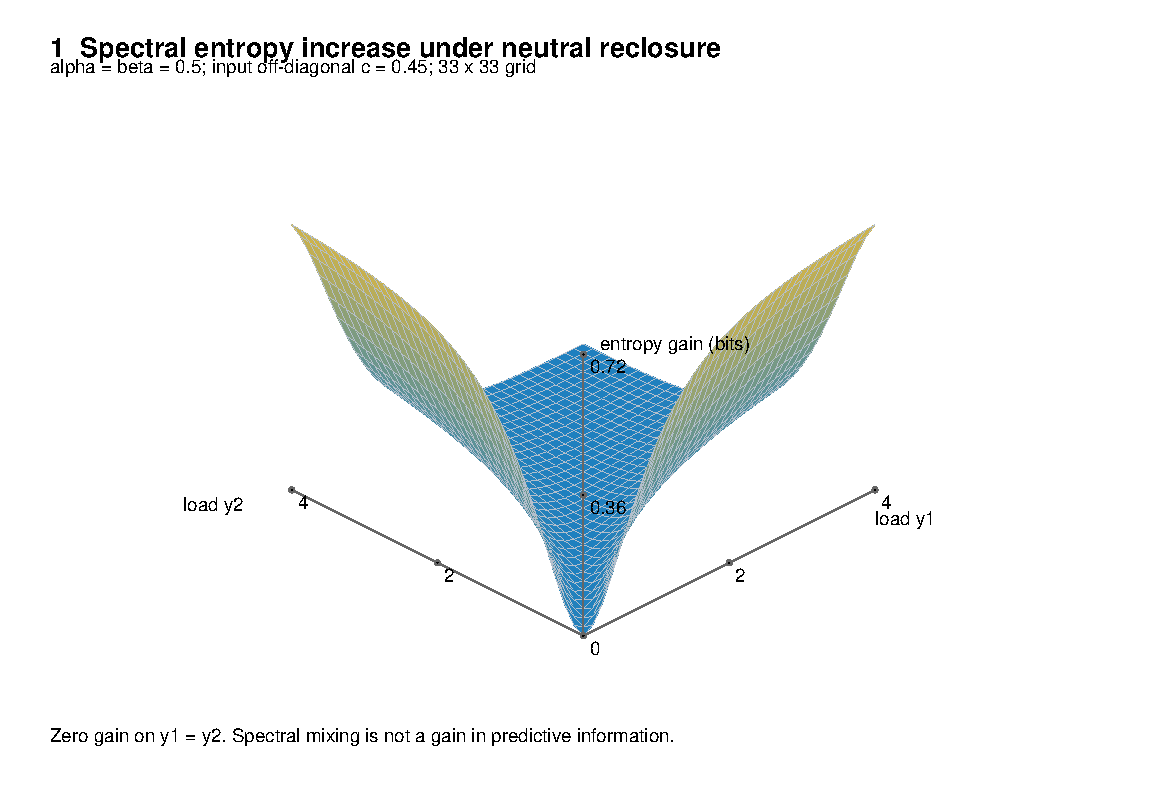
\includegraphics[width=\linewidth]{figures/figure_1_entropy_surface.pdf}\par\small\itshape Figure 1. Three-dimensional spectral-entropy increment for Equation (13), c=0.45, alpha=beta=0.5 and y\_1,y\_2 in [0,4]. The 33 x 33 grid has exact zero increment on equal-load states. This is a deterministic mathematical surface, not biological measurements.\end{figure}
\section*{7.3 Predictive growth requires a separate endpoint}
Proposition 4 prevents a deterministic BFG feature from adding information beyond its complete input history. A separate acquired measurement W can, in principle, add conditional information I(Y\_future;W|X\_history); this must be estimated and tested using an independently defined future target. Increased knowledge from additional observations differs from growth of a molecular or organizational capacity. Likewise, increased spectral entropy measures greater eigenvalue mixing, not necessarily more target-relevant distinguishability. A biological information-growth claim must specify the evolving distribution, the target, the measurement channel and a capable rival.

An exact direct implementation rho\_next=Chi circ rho reproduces every output of the declared polar construction. In the synthetic setting this control is an algebraic clone, not a separately fitted biological alternative. It establishes that observed successor matrices alone cannot select the factorization as a unique physical mediator. A selective intervention and an independently measured mediator are required for that stronger claim.

\section*{8 Reproducible numerical illustrations}
\section*{8.1 Computational specification}
All new numerical examples are constructed in this manuscript. The damage model in Equations (7)-(10) uses u\_D=0 after an initial burden D(0)=2, constant repair r and constant p21 degradation; no chromatin parameter or future cell-cycle information enters. Initial P,M,Q and the pre-zero delay history are the damage-free fixed point: (0.110998797,0.050455332,0.134142813). We integrate to model time 80 with fourth-order Runge-Kutta steps of 0.01 and linear interpolation of the stored delayed p53 history. A step-halving calculation uses 0.005. For positive delay 2, all interpolated points precede the current step. For delay zero, the current Runge-Kutta stage is used. The interpolation makes the delayed solver distinct from a fourth-order accurate delay integrator.

\begin{longtable}{p{7.9cm}|p{7.9cm}}
Parameter group & Dimensionless values\\\hline
p53: sP, kD, KD, deltaP, kM & 0.05, 2, 0.5, 0.4, 1\\\hline
MDM2: sM, kP, deltaM & 0.02, 1.2, 0.4\\\hline
p21: sQ, kQ, deltaQ & 0.02, 0.8, 0.15\\\hline
Hill h, K; tau; repair r & 4, 1; {0,2}; {0.12,0.03}\\\hline
\end{longtable}{\small\itshape Table 3. Illustrative parameters selected for model contrasts; none are estimated molecular rates.\par}
The CSV files also contain illustrative organizational readouts: E\_exp=1+D, E\_bind=(1+Q)/(1+Q\_base), I=(1+P)/(1+P\_base), I\_0=1 and Phi=E\_exp I/E\_bind. These choices force the damage-free reference to Phi=I=1. They are declared normalized indices, not physical energies or Shannon information. IB is the numerical time derivative of Phi I using centered differences in the interior and second-order one-sided endpoint formulas. The plots use D,P,Q themselves; no organizational readout is used to infer a biological fate.

\section*{8.2 Response contrasts and integration checks}
\begin{longtable}{p{2.63cm}|p{2.63cm}|p{2.63cm}|p{2.63cm}|p{2.63cm}|p{2.63cm}}
Case & tau & r & max P & max Q & D(80)\\\hline
A & 0 & 0.12 & 1.4053 & 1.7053 & 0.000135\\\hline
B & 2 & 0.12 & 2.4501 & 2.2766 & 0.000135\\\hline
C & 0 & 0.03 & 1.4236 & 2.1697 & 0.181436\\\hline
D & 2 & 0.03 & 2.5287 & 2.3411 & 0.181436\\\hline
\end{longtable}{\small\itshape Table 4. Computed synthetic responses; maxima are sampled on the 0.01 time grid.\par}
Adding delay raises the first sampled p53 maximum from 1.4053 to 2.4501 for r=0.12 and produces further damped excursions in these selected traces. Lowering repair leaves D(80)=0.181436 instead of 0.000135457; the damage trajectory itself is independent of delay because repair is constant here. The exact solution D(t)=2 exp(-rt) agrees with integration within 1.27 x 10^-14. The largest all-state difference between the displayed and half-step trajectories at shared times is 4.83 x 10^-6 in delayed case B, and below 2.28 x 10^-10 without delay. This checks numerical consistency over the specified horizon, not empirical parameter accuracy or global stability.

\begin{figure}[htbp]\centering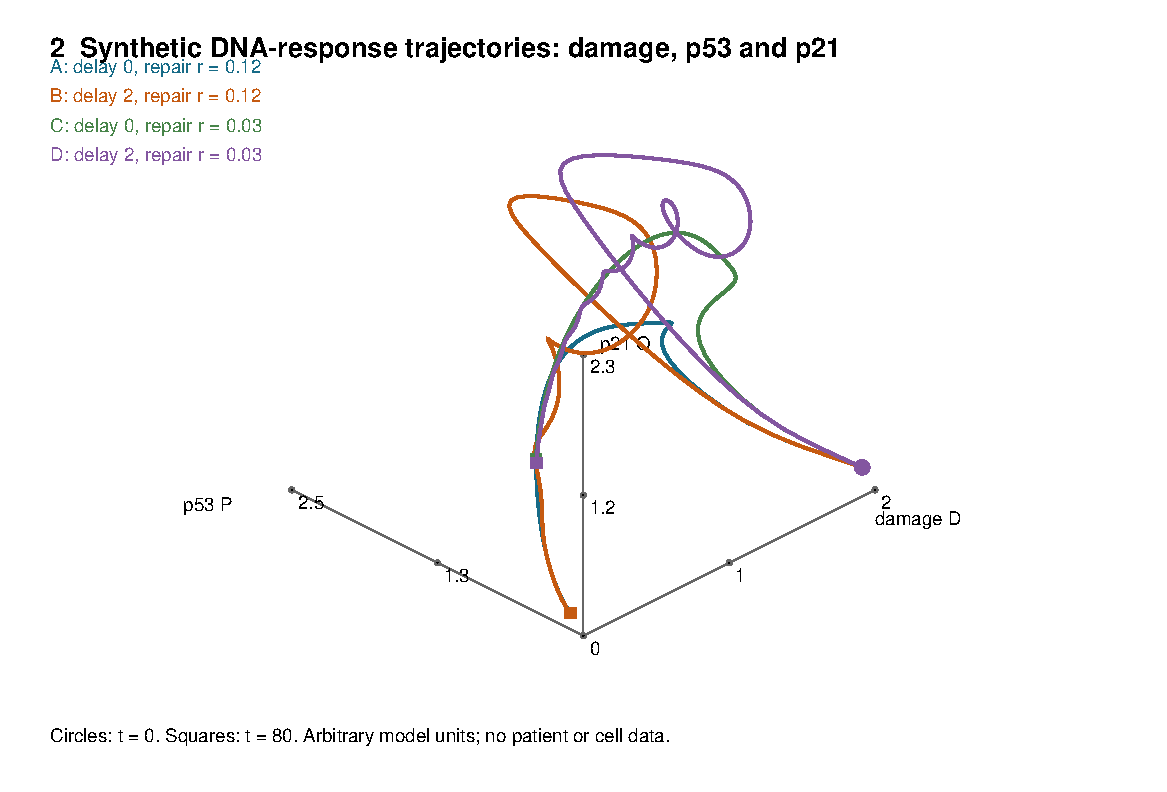
\includegraphics[width=\linewidth]{figures/figure_2_phase_trajectories.pdf}\par\small\itshape Figure 2. Three-dimensional projected paths in damage, p53 and p21 coordinates for four synthetic cases. All paths begin at the same initial state. Circles and squares identify the start and end. The projection is illustrative; Figure 3 supplies the temporal context.\end{figure}
The trajectories return at different rates; case C or D can remain far from the damage-free condition during the chosen horizon. That finite observation does not establish permanent arrest or senescence. The model has no mitosis event mechanism, death state or senescence assay. It cannot generate valid counts of biological recovery, nor demonstrate predictive superiority of BFG.

\section*{8.3 Operator audit and inheritance controls}
The operator audit uses seed 20261001 and 1,000 independent complex 3 x 3 matrices X with normal real and imaginary entries. We form rho=XX-dagger/tr(XX-dagger), draw three loads uniformly on [0,4], and draw alpha uniformly on [0.1,0.9]. The polar-isometry construction and the explicit Schur multiplier agree with maximum absolute entry error 3.33 x 10^-16. The second-moment identity has maximum absolute residual 2.43 x 10^-16. All sampled entropy increments are nonnegative, with a minimum 6.78 x 10^-7 bits. These are implementation audits of fixed identities; random-trial frequency is not a physical probability.

Equal-load and diagonal-state controls are exact analytically, since chi=1 on equal-load blocks and diagonal entries never change. With the two-state loads (0,2) frozen, c\_n=0.45 chi^n approaches zero and entropy approaches one bit, so the construction saturates rather than generating unlimited entropy. The bounded recurrence uses initial q\_0=q\_1=1. Coefficients (a,b,s)=(0.5,0.25,0.1) approach 0.4; (0.6,0.35,0.1) approach 2. The latter reaches only 1.51326 at n=20. The uncontrolled Fibonacci comparator reaches 10,946 at n=20. No common information unit is assigned to these scalar trajectories.

\begin{figure}[htbp]\centering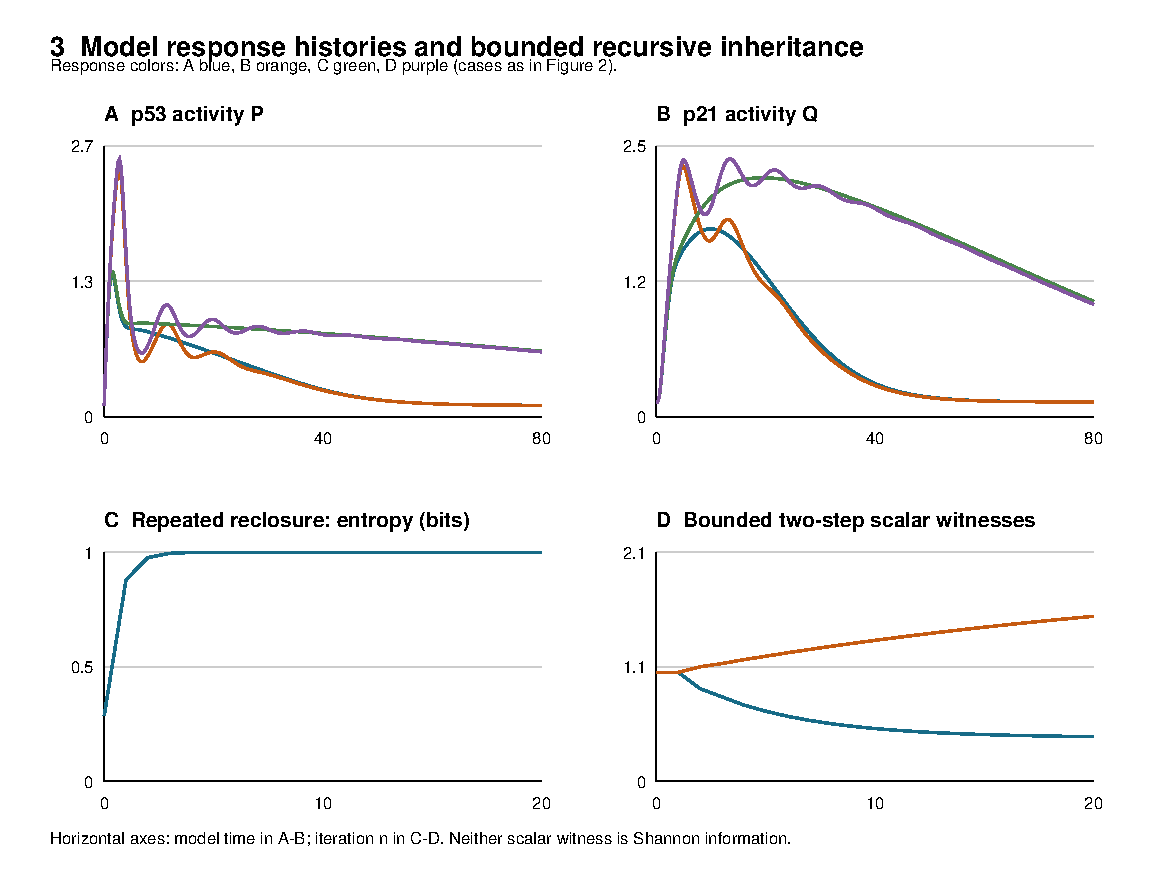
\includegraphics[width=\linewidth]{figures/figure_3_temporal_responses.pdf}\par\small\itshape Figure 3. Computed temporal response histories (A,B), repeated two-state spectral entropy (C), and two bounded inheritance witnesses (D). The blue and orange curves in panel D denote its two coefficient sets, not the response cases. The Fibonacci control is retained in the raw results and omitted from panel D because its unbounded scale would obscure the bounded trajectories.\end{figure}
\section*{9 Defining regulatory return and a prospective comparison}
Regulatory return should be measured relative to a reference set for a specified cell type, environment and cell-cycle phase. Let z(t) be an independently chosen multivariate witness, A\_ref($\psi$) its reference set and $\Sigma$ a positive-definite covariance estimate obtained in training data. One candidate return distance is

\begin{equation}R(t)=\inf_{a\in\mathcal A_{\mathrm{ref}}(\psi(t))}\left[(z(t)-a)^\top\Sigma^{-1}(z(t)-a)\right]^{1/2}.\tag{14}\end{equation}
This is a proposed measurement definition, not a validated identity score. A sustained return criterion requires R below a training-derived threshold over a declared dwell interval, with viability assessed separately. Reference sets accommodate normal cycling trajectories; forcing every phase toward a single static centroid would incorrectly label normal variation as failed recovery. The witness, covariance regularization and threshold must be frozen before evaluating held-out experiments.

The primary prediction task begins at a landmark time after damage input. Only observations available by that time enter the predictor. The outcome is time to the next verified division, or division within a fixed future horizon. Cells already dividing before the landmark require an explicit inclusion rule. Tracks ending before the horizon are censored rather than assigned to permanent arrest. Mother-daughter lineages, shared imaging fields and experimental batches must remain within the same validation partition where dependence would otherwise cause leakage.

Three comparisons are required. M0 is a biologically motivated damage and p53-MDM2-p21 model. M1 uses the same observations but applies fixed BFG features or cross-condition constraints. M2 is a suitable statistical predictor using the original multivariate history and ordinary temporal features. A comparison with a snapshot-only predictor provides a useful lower baseline but cannot establish that BFG improves on existing dynamic descriptions.

For a binary division outcome at the declared horizon, one primary score can be the paired difference in held-out log predictive density:

\begin{equation}\Delta L=\sum_{i\in\mathcal D_{\mathrm{test}}}\left[\log p_{M1}(Y_i\mid X_i)-\log p_{\mathrm{rival}}(Y_i\mid X_i)\right].\tag{15}\end{equation}
Calibration, prediction intervals where relevant and errors by condition accompany the primary score. Hyperparameters, smoothing, feature selection and normalization are learned within training partitions. Uncertainty should reflect independent experimental units and lineages. Prospective external transfer uses frozen transformations; any adaptation rule must be declared. Sample size and a practically relevant improvement threshold remain design choices to establish before an empirical study. No numeric threshold or power estimate is invented here.

\section*{10 Hypotheses and discriminating tests}
H1 concerns recovery beyond scalar balance. Conditional on a scalar $\Phi$, separate regulatory channels and past response history predict future division or regulatory return. The test compares M1 and M2 with scalar-only models on held-out experiments. Failure of the scalar model is consistent with Proposition 3, but successful multivariate prediction is not specific evidence for BFG.

H2 concerns the contribution of the BFG restriction. Prespecified organizational readouts or constraints improve prediction, calibration or transfer relative to both M0 and an appropriately capable M2. Improvement should survive reasonable changes in proxies and smoothing and a comparison of model complexity. If gains occur only against a weak snapshot comparator, the additional BFG claim is unsupported. Equal performance may still support a compact description, but must be reported as such.

H3 concerns separation of endpoints. Regulatory return and resumed proliferation need not coincide. A cell may occupy a stable viable state without dividing during the outcome window. This requires measuring both outcomes, rather than defining return using division and then presenting their association as a discovery. Classification of longer-term senescence remains a separate study requiring its own evidence.

H4 concerns noncoding regulatory context. A measured or selectively perturbed context changes restoration or coupling in ways that predict transfer between conditions. This extension requires appropriate chromatin, regulatory or intervention measurements; p53 and p21 trajectories alone do not identify noncoding architecture. Comparators must allow ordinary regulatory-context effects, and interventions must be assessed for off-target changes. A fitted context coefficient is not evidence of a unique neutral mediator.

\section*{10.1 Data access and analysis boundaries}
The published analysis by Gutu et al. [13] points to earlier studies for underlying data and provides an analysis-code link. Tran et al. [12] provide a code link and state that supporting data are available on request. These statements identify possible access routes, not a completed data acquisition. No raw tracks have been downloaded, reanalyzed or licensed for redistribution in this work. Any subsequent study must record dataset versions, reporter definitions, inclusion rules and access terms before fitting.

Destructive single-cell assays and live trajectories cannot be treated as simultaneous repeated measurements from the same cell unless the experimental design provides that linkage. A terminal damage marker is unavailable at an earlier prediction landmark and cannot enter an early predictor. If paired chromatin and live response measurements are unavailable, H4 must remain outside the first empirical analysis. Lack of the necessary measurements is a scope limit rather than grounds for replacing the missing biology with an arbitrary proxy.

The reported work combines analytical results, synthetic numerical illustrations and a prospective protocol. It is not an executed preregistered biological study. A future registration must fix the dataset, observation model, transformations, failure criteria and validation partitions before reporting predictive superiority.

\section*{11 Discussion and conclusion}
The BFG source corpus offers a common language for persistence through change, but a useful cellular theory must resolve the relation between its organizational quantities and measured biology. This paper makes that relation explicit at three levels. The source ratio is a candidate summary. The reduced equations imply particular mathematical dynamics. The proposed DNA response specialization supplies additional molecular states and observational assumptions. None of these levels can substitute for the others.

Proposition 2 identifies a concrete gap between the reduced dynamics and pulse-based response descriptions. Proposition 3 establishes that scalar balance and a vanishing information derivative cannot generally identify functional recovery. Proposition 4 explains why predictive improvement from derived BFG features should be interpreted as the value of a representation or inductive restriction, until independent mechanistic evidence supports more. These results narrow the claims while making the next comparison testable.

The prospective framework also distinguishes maintenance of a cell from maintenance of a tissue. Removal of a damaged cell may benefit tissue organization while terminating that cell. The source discussion of organism-level export or apoptosis [3,4] therefore cannot label cell death as successful single-cell identity preservation. A multiscale extension would need separately defined cell and tissue outcomes and measured coupling between them.

The main limitation is the absence of empirical model fitting and prospective validation. The synthetic delayed model demonstrates responses under chosen parameters, but has not been fitted to a dataset and does not reconstruct upstream ATM/Wip1 initiation or a senescence mechanism. The positive operator specialization has no identified cellular observation map. Regulatory return depends on a witness and reference set. Noncoding-context tests require additional measurements. The conditional results and numerical checks do not validate BFG as a general biological theory.

The next research step is a comparison of future division predictions and independently measured regulatory return, using a documented single-cell dataset and fixed transformations. Only if that comparison succeeds should the study expand to chromatin context, persistent state transitions or tissue-level regulation. The resulting claim would concern a specified task and model class. It would not establish a universal repair principle or a therapeutic recommendation.

\section*{12 Reproducibility and declarations}
The numerical supplement contains executable reproduction code, exact parameter settings, four time-series CSV files, operator-audit rows and frozen results. Three figures are supplied as vector PDF and high-resolution PNG. The analytical claims are conditional on their displayed assumptions; the numerical work is synthetic. The source manifest records file hashes and used locations. External bibliographic records were checked against publisher, PubMed or author-maintained scholarly pages on 1 October 2026. No external raw biological tracks were downloaded or redistributed.

AI assistance was used for source retrieval, synthesis, mathematical drafting, numerical code and document preparation. Marcel Theodor Wende is the proposed author; final author approval and submission-specific funding and competing-interest statements remain for author completion. Coauthored precursor works retain their own authorship and do not imply coauthorship or endorsement here. No human or animal participant data were processed.

\clearpage
\section*{Appendix A. Notation and conditional scope}
\begin{longtable}{p{7.9cm}|p{7.9cm}}
Symbols & Meaning\\\hline
Phi, I, IB & Order index, structured index, derivative of their product\\\hline
C\_n, N\_n, E\_n, X\_n & Source closure, mediator, export and context roles\\\hline
m\_n, G\_n, q\_n & Chosen magnitude, closure gain, new bounded scalar witness\\\hline
D, P, M, Q & Effective damage, p53, MDM2 and p21 states\\\hline
Y, rho, Chi, T & Load, positive unit-trace state, Schur matrix and map\\\hline
R, Y\_future, Delta L & Reference distance, independent future outcome, test-score difference\\\hline
\end{longtable}{\small\itshape Table A1. Symbols are not interchangeable between their source and applied state spaces.\par}
Proof dependencies: Proposition 2 uses only the constant-coefficient autonomous logistic system. Proposition 3 uses the proxy-map row-space condition, not a biochemical trajectory. Proposition 4 uses a fixed deterministic transform of the complete history. Proposition 1 uses nonnegative coefficients with a+b<1. Proposition 5 uses the positive two-state specialization of the source multiplier and unequal loads. None of these propositions identifies a physical DNA mediator. The general entropy statement uses standard unital-channel majorization [19].

\section*{Appendix B. Computational and source provenance}
Run numerical\_supplement/reproduce.py with Python, NumPy, ReportLab and pypdfium2 from the package directory or any working directory. Output paths are resolved relative to the supplied script. It regenerates numerical results and figures without downloading data or contacting an account. CSV trajectories retain every displayed-grid sample; maxima and errors are recorded in results.json. The code checks positivity and finite trajectories, the analytical damage solution, the polar/Schur equivalence, the moment identity and sampled entropy increments. IB endpoint estimates are finite-difference values, not a separately integrated state.

Used BFG locations: [1] pp. 4-11 and Appendix C; [2] pp. 5-11; [3] pp. 120-122, 172-174 and 187-189; [4] paragraphs 8,14,21 and Table 32 in the DOCX extraction; [5] Sections 6-10; [6] Sections 7-9, 16.4 and 17.5; [7] growth and Balance-Field commentary, including extracted paragraphs 638-647 and source crosswalk; [8] Sections 10-12; [9] Sections 2-7. PDF page indices refer to supplied files. Original manuscripts are cited for provenance; they are not redistributed in the supplement.

\clearpage
\section*{References}
References [1-9] document BFG source provenance. References [10-21] are external scholarly sources checked online; they supply biological evidence or established mathematical tools, not independent confirmation of BFG.

[1] Wende MT. Resolving the DNA Gene-Regulation Problem as a Stability-and-Feedback Question in the Balance-Field Framework (BFG): A Fully Operational, Mathematical, and Physically Interpretable Whitepaper. Author manuscript. 5 March 2026.

[2] Wende MT. The Function of Non-Coding DNA as Regime Architecture: A Fully Operational, Mathematical, and Physically Interpretable Resolution in the Balance-Field Framework (BFG). Author manuscript. 5 March 2026.

[3] Wende MT. BFG Model of Biological Organism Formation. Supplied author monograph. Source sections on homeostasis, identity transport and regeneration; publication status not independently established.

[4] Wende MT. BFG Biological Organism Formation: Trinity, Level 0 and AGC Integrated Journal-Ready manuscript. Supplied author manuscript. The filename indicates a preparation label, not acceptance or publication.

[5] Wende MT. Multiscale Neural Organization and Conscious Closure in the Balance Field Framework. Preprint version 1.0. 1 October 2026.

[6] Wende MT. The Recursive Closure Growth Principle: A Fibonacci-Like Architecture for Multi-Scale Stability, Trinitarian Mediation, and Emergent Closure Hierarchies within the Balance-Field Framework. Author whitepaper. 2026.

[7] Wende MT. Trinitarian Recursive Closure Architecture: A Pure Balance-Field Framework Monograph. Strongest Integrated English Edition. Supplied author monograph; public publication status not independently established.

[8] Wende MT. Canonical Minimal Finite Closure and Universal Reclosure in the Balance-Field Framework. Supplied preprint. 26 September 2026.

[9] Wende MT. Balance-Field Framework (BFG): Canonical Reclosure and Structural Novelty. Mathematical preprint. 22 September 2026.

[10] Lahav G, Rosenfeld N, Sigal A, Geva-Zatorsky N, Levine AJ, Elowitz MB, Alon U. Dynamics of the p53-Mdm2 feedback loop in individual cells. Nature Genetics. 2004;36:147-150. https://doi.org/10.1038/ng1293

[11] Purvis JE, Karhohs KW, Mock C, Batchelor E, Loewer A, Lahav G. p53 dynamics control cell fate. Science. 2012;336(6087):1440-1444. https://doi.org/10.1126/science.1218351

[12] Tran AP, Tralie CJ, Reyes J, et al. Long-term p21 and p53 dynamics regulate the frequency of mitosis events and cell cycle arrest following radiation damage. Cell Death and Differentiation. 2023;30:660-672. First published online 1 October 2022. https://doi.org/10.1038/s41418-022-01069-x

[13] Gutu N, Binish N, Keilholz U, Herzel H, Granada AE. p53 and p21 dynamics encode single-cell DNA damage levels, fine-tuning proliferation and shaping population heterogeneity. Communications Biology. 2023;6:1196. https://doi.org/10.1038/s42003-023-05585-5

[14] Shannon CE. A mathematical theory of communication. Bell System Technical Journal. 1948;27:379-423,623-656. https://www.nokia.com/bell-labs/publications-and-media/publications/a-mathematical-theory-of-communication/

[15] Cover TM, Thomas JA. Elements of Information Theory. 2nd ed. Wiley; 2006. https://doi.org/10.1002/047174882X

[16] Pattee HH. The physics of symbols: bridging the epistemic cut. BioSystems. 2001;60(1-3):5-21. https://doi.org/10.1016/S0303-2647(01)00104-6

[17] Ciliberto A, Novak B, Tyson JJ. Steady states and oscillations in the p53/Mdm2 network. Cell Cycle. 2005;4(3):488-493. https://doi.org/10.4161/cc.4.3.1548

[18] Batchelor E, Mock CS, Bhan I, Loewer A, Lahav G. Recurrent initiation: a mechanism for triggering p53 pulses in response to DNA damage. Molecular Cell. 2008;30(3):277-289. https://doi.org/10.1016/j.molcel.2008.03.016

[19] Watrous J. The Theory of Quantum Information. Cambridge University Press; 2018. Chapters 4-5. Author-maintained manuscript and bibliographic page: https://cs.uwaterloo.ca/~watrous/TQI/

[20] Gorgoulis V, Adams PD, Alimonti A, et al. Cellular senescence: defining a path forward. Cell. 2019;179(4):813-827. https://doi.org/10.1016/j.cell.2019.10.005

[21] Jackson SP, Bartek J. The DNA-damage response in human biology and disease. Nature. 2009;461:1071-1078. https://doi.org/10.1038/nature08467

\end{document}